\documentclass{article}
% uncomment the line below if you like. You may lack dependencies if you do.
%\usepackage{proposal}
\usepackage{tikz,mathpazo}
\usetikzlibrary{shapes.geometric, arrows}
\usepackage{flowchart}
\usepackage{graphicx}

\usepackage{url}
\parindent 0pt \parskip 2pt
\title{EE 586L Kinetetris}
\author{Hengyue Liu, Jason Pang, Yihao Xia}
\begin{document}
	\maketitle
	
	
	\section{Abstract}
	Our project aims to develop a real-time image processing based Tetris game that can be competitive for 1-2 players. Essentially the player(s) can begin and play Tetris using hand gestures and arm motions, within a bounding box, that are visually captured using either a camera or a Kinect, and the game ends when the blocks are stacked above a certain height for the player. In the 2 player competitive mode, an additional element of random difficulty is added when clearing lines on one side generates random block drops on the other.
	
	\section{Description of the system}
	Our system includes (per player) a DSP board, camera, speakers, and a screen. The cost of a DSP board is around \$30 \cite{price}, Kinect costs around \$70 (used) to \$115 (new), monitors can vary in price from \$15 to \$100+, and speakers can also vary from \$20 to \$100+, depending on the output quality (e.g. monitor resolution, sound quality). Then there are various cables to link the DSP board with the other components. Altogether this makes for a rather expensive prototype if one were to want to market the game. One interesting possibility for the system would be as part of an arcade game, where it would serve as something for groups of people to play together casually, and the hardware cost could then be covered by the arcade owner, since it seems unlikely that masses of people would want to own so much hardware (which also makes it difficult to port around).\\
	
	Here is a simple flowchart for the prototype of the whole system:\\
	\begin{figure}
		\begin{center}
			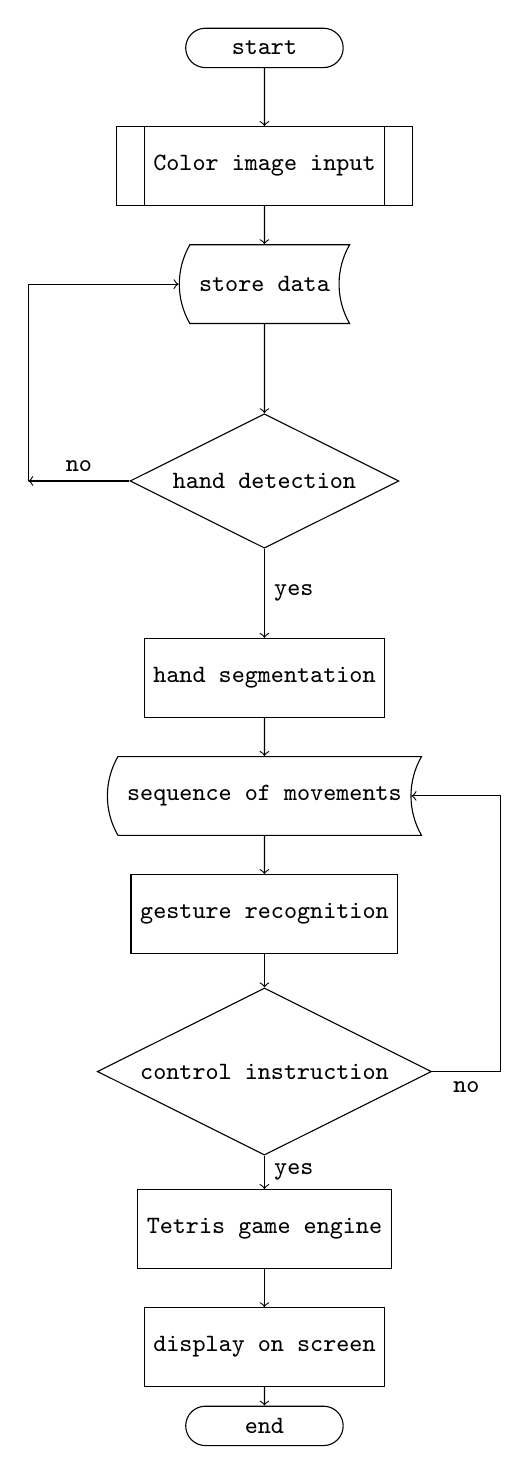
\begin{tikzpicture}[font={\sf \small \ttfamily}]
			\def \smbwd{2cm}
			\thispagestyle{empty}
			\node (start) at (3,0) [draw, terminal,minimum width=\smbwd, minimum height=0.5cm] {start};      % ???? 
			\node (getdata) at (3,-1.5) [draw, predproc, align=left,minimum width=\smbwd,minimum height=1cm] {Color image input};        %????????????
			\node (decide) at (3,-5.5) [draw, decision, diamond, aspect=2, minimum width=\smbwd, minimum height=1cm] {hand detection};    %??????
			\node (storage) at (3,-3.0) [draw, storage, minimum width=\smbwd, minimum height=1cm] {store data};     %??????
			\node (step1) at (3,-8.0) [draw, process, minimum width=\smbwd, minimum height=1cm] {hand segmentation};      %??????
			\node (step2) at (3,-11.0) [draw, process, minimum width=\smbwd, minimum height=1cm] {gesture recognition};      %??????
			\node (store2) at (3,-9.5) [draw, storage, minimum width=\smbwd, minimum height=1cm] {sequence of movements};
			
			\node (instruction) at (3,-13.0) [draw, decision,diamond, aspect=2, minimum width=\smbwd, minimum height=1cm] {control instruction};
			\node (game) at (3,-15.0) [draw, process, minimum width=\smbwd, minimum height=1cm] {Tetris game engine};  
			\node (display) at (3,-16.5) [draw, process, minimum width=\smbwd, minimum height=1cm] {display on screen};      
			\coordinate (point1) at (6,-13.0);
			\coordinate (point2) at (0,-5.5);
			
			\node (end) at (3,-17.5) [draw, terminal,minimum width=\smbwd,minimum height=0.5cm] {end};
			\draw[->] (start) -- (getdata);
			\draw[->] (getdata) -- (storage);
			\draw[->] (storage) -- (decide);
			\draw[->] (decide) -- node[right]{yes} (step1);
			\draw[->] (decide) -- node[above]{no}(point2);
			\draw[->] (point2) |-(storage);
			\draw[->] (step1) -- (store2);
			\draw[->] (store2) -- (step2);
			\draw[->] (step2) -- (instruction);
			\draw[->] (instruction) -- node[right]{yes}(game);
			\draw[->] (instruction) -- node[below]{no}(point1) |- (store2);
			\draw[->] (game) -- (display);
			\draw[->] (display) -- (end);
			
			\end{tikzpicture}
		\end{center}
		\caption{game system flowchart}
	\end{figure}
	\newpage
	Here is a simple flowchart for the game engine:\\
	\begin{figure}[h!]
	\centering\includegraphics[scale=0.55]{tetrisproject}
	\caption{game engine flowchart}
	\end{figure}
	\newpage
	Game description: two simultaneous games of Tetris in 10x20 block grids on a split screen. Whenever a player clears a certain number of lines (e.g. clearing a total of 10x lines), random blocks get dropped into the opposing player field after a brief warning delay. In between the two screens is a center margin, where the stats from each screen will track the number of lines cleared. This region will also have a cartoon image of what each current player’s gestures are being read as. For example, a regular hand sign will indicate the default non-action move, a clockwise arrow will indicate rotation to the right, a counter-clockwise arrow will indication rotation to the left, and a flashing down arrow will indicate a block drop. The horizontal position of the block will be tracking the player hand positions. If we play over a desk (as a backup option) instead of in front of a screen, then the player horizontal hand position will instead indicate whether to move the blocks left or right (as well has how fast, scaling faster the longer the hand is displaced from the center). When a block is placed the exceeds the maximum grid height on either side, the game ends and the opposing side is victorious.\\ 
	
	\section{Description of Possible Algorithms}
	If we want to include a computer opponent, we could also write a Tetris solving algorithm \cite{ai}. The algorithm would attempt to search (to a certain depth level) the ideal move for a particular tetronimo (4 block piece) within calculation restraints, and perform the move based on that. The speed or delay of the algorithm, and the depth of the search would scale with the difficulty level of the AI.
	
	%-algorithm for extracting hand/arm movements/gestures
	\begin{itemize}
		\item{Hand detection}
		
		We will use a color camera, so the players can have their hands on a desk or somewhere with single-colored background. Under ideal lighting, we could use envelope detection to get the outline of the hand, and track that. Alternatively, we could track the center of the hand, as well as the 5 fingertips, to make gesture recognition easier.If we have the player play over the output screen, we will need to also segment out their body. A promising approach is to use multi-feature fusion and template matching \cite{multifeaturefusionarticle}. The template matching aspect is more vital for gesture recognition, as below.\\
		\item{Gesture recognition}
		
		For hand gesture recognition step, two techniques are used. One is dissimilarity measure, another is template matching \cite{ren2011robust}. We keep track of the hand variations between frames, the hand movement of one certain complete gesture will give a unique pattern of variations, then use that as a template. By calculation the similarity of this pattern, compare it to the template, if it is acceptable (within the thresholds), then the sequence of hand movement  can be matched to certain gesture. While we don’t know how viable it is, with enough training data, we might be able to obtain a robust template for gesture recognition.\\
		
		The hand gestures recognition contains both spatial and temporal gesture segmentations, to determine where and when the gesture occurs. We need to establish a framework to segment the hand gesture spatially and temporally. To recognize the hand gesture, we need to extract the features of different gestures by employing some pattern recognition algorithm and then build a gesture models for incoming gesture recognition.\\
	\end{itemize}
	
	\section{Complexity Analysis}
	The system will need to handle images at a rate that balances detail and memory capacity/ processing speed.We’re going to aim for a rate of 15 frames per second at first, and then tweak it up if the system runs perfectly well, or lower it if the system struggles. Most of the memory will probably be taken up by a buffer (or buffers) that stores all the image data that are processed or going to be processed. We also will need to use the processed results to recognize gestures, swipes, etc., as moves, and write game code that runs at a realistic pace. In addition, we will probably have to write a game AI for computer players, and this AI will likely take up a fair amount of computational power to perform searches for the best moves (e.g. up to a depth of 2 moves ahead), and then perform these moves at a particular speed to simulate player difficulty. We might also incorporate random AI errors to simulate occasion “human” behavior.\\
	
	In addition, a robust gesture recognition will likely require additional ‘non-gesture’ recognition to prevent false recognition, for example if a movement resembles more than one gesture, we may need to either ignore the movement until the player makes the movement clearer , or allow for weighting so that the system will perform only the closest similarity gesture in the case of a majority (e.g. 80\% similar to one gesture and 20\% similar to another).\\
	
	\section{Major Challenges}
	Optimization, how to omit unintended moves, how to deal with the sub-gesture problem, how to recognize multiple hand gesture.\\
	
	Sub-gesture Problem: false detection of gestures that are similar to parts of other longer gestures.\\
	
	One major challenge that we are likely to encounter is: how fast can we run the game? In order to make the system more sensitive to intricate player movements, we have to incorporate more data, such as in the form of more frames per second. However, this will make the system more memory and processor intensive. On the other hand, if we don’t try to obtain a system that’s as fast as possible, players might notice or experience a lag in the gameplay, which would be very undesirable. Besides, allowing multiple candidates in the game increase computational time require us to further optimize the algorithm.\\ 
	
	Another foreseeable challenge is figuring out not just how to recognize proper moves (such as moving blocks left/right, dropping blocks, rotating them), but also how to exclude unintentional moves (such as an arm movement that is part of a natural sway, or drifting position from fatigue, or ambiguous movements that could be meant for one type of move but is actually intended to signify another type of move). Various factors of the background would cause problems including changing illumination, low-quality video (tradeoff of calculation time), temporary occlusion, and background clutter.\\
	
	Different users can perform movements at different speeds, so another challenge is figuring out the start and end of a gesture. When a user makes a move, for example swiping right for moving one block to right, at the end of this gesture, the hands will return to its original position afterwards, i.e. moving left. So, we can consider this change in frames to be the end of the gesture. In other words, if we assume the user has one or more preferred ‘default position(s)’ then any return to default indicates that an action choice such as swiping has just been completed.\\
	
	
	\section{Modeling Tasks}
	We need to model the computer AI speed and how to control it to simulate real-time behavior (e.g. a novice computer would take a long time to make moves, while a master computer would make Tetris decisions quickly).\\
	\section{Human Factors}
	User evaluation will be based on a few things, focusing on balancing the challenge of the game with its enjoyment. For the challenge aspect, we want to be able to scale the difficulty for all skill levels (from easy to master). This is the most important part, because a game that is too difficult to play will be hard to enjoy because of the lack of progress, but a game that is too easy to play will be boring. Thus we will probably develop difficulty tiers and test it out by having various skill level players evaluate whether those tiers are suitably difficult and enjoyable (not just for themselves, but also for what they believe is suitable at those particular levels).\\
	
	Another important human factor is that gesture recognition must be suitable for the vast majority of players (unfortunately there are cases that the system probably cannot be played, for example by someone who doesn’t have any hands). This means that what the majority of humans recognize as a gesture should also be recognized as a gesture by the algorithm, regardless of any other variation in gestures between different people. Also, not just gesture variation between people, but also gesture variation for a single person over time (due to fatigue or other factors).\\
	
	
	\section{Training}
	We will need to design various levels of computer AI and optimize their behavior within certain standards. Training data set can be obtained by having various volunteers of different skill levels play the game, and in addition to measuring their performance against AI or other people, also request their feedback for how appropriate they felt the game and/or AI skill levels to be.\\
	
	\section{Rough schedule}
	\renewcommand\labelenumi{(\theenumi)}
	\begin{enumerate}
		\item{video input and data extract}
		\item{real time gesture recognition}
		\begin{itemize}
			\item{hand detecting}
			\item{gesture modeling}
			\item{gesture recognition}
		\end{itemize}
		\item{game design}
		\item{optimization (might take a long time)}
		\item{quality of life improvements (visual/ audio quality improvements, user interface improvements, appeal)}
	\end{enumerate}
	
	\section{Final Test Set-Up} 
	Demo scenario- camera either facing the players, or pointed down at a tabletop with marked boundaries. We will first aim for a scenario in which the players play in front of a screen, with the camera observing the player’s hand before the screen. The camera input is (in terms of pixels), 480 height by 720 width, so the we can divide the halves as having two 480x240 Tetris games on the left and right side (with 24x24 pixel blocks), and the center 480x240 region displaying player statistics.\\
	
	Output- split screen with Tetris game and feedback on both sides, speakers for music/sound effects.\\
	\section{Board}
	Need: DAVINCI TMS320DM6437 EVM, as well as a camera (Color TeleCamera, model number NCK 41CV), a screen to display the game, and probably speakers for background music and sound effects.\\ 
	
	\section{References}
	
	\bibliographystyle{plain}
	\bibliography{references}
	
	
	
\end{document}



